\chapter{Dagli NPC tradizionali agli LLM: background e stato dell'arte}

\section{NPC tradizionali: analisi e limiti}

L'IA nei videogiochi è nata praticamente in simbiosi con i videogiochi stessi. Basti pensare a \textit{Pong}\cite{pong}, in cui l'avversario deve cercare di colpire la pallina evitando di subire punto. Un altro esempio importante è \textit{Pac-Man}\cite{pacman} del 1980, dove i quattro fantasmi hanno ciascuno un algoritmo differente per raggiungere il protagonista: Blinky, il fantasma rosso, imposta il suo obiettivo di movimento in base alla posizione attuale di Pac-Man, mentre Inky, il fantasma blu, si basa sulla posizione del fantasma rosso e di Pac-Man per accerchiarlo.
Inizialmente gli NPC servivano principalmente per dare una sfida al giocatore. Oggi troviamo sistemi più complessi, alcuni dei quali simulano anche il comportamento umano, come \textit{The Sims}\cite{thesims}, che simula la vita quotidiana delle persone. Come osserva Millington: ``Now we have a massive diversity of AI in games. Many genres are still using the simple AI of 1979 because that's all they need'' \cite{millington2019artificial}. Nonostante l'IA nei videogiochi, e più in generale nel mondo dell'informatica, si sia evoluta molto, vari videogiochi moderni utilizzano ancora strutture vecchie di decenni. Il motivo risiede nella diversità dei generi videoludici e nello scopo che ogni videogioco si prefigge, come già introdotto nel Capitolo 1.
Normalmente un'IA per un NPC viene strutturata in tre moduli principali: movimento, decision making e strategia, come mostrato in Figura \ref{fig:moduli_ia}. Questa è una struttura proposta da Ian Millington per spiegare meglio il concetto di IA nei videogiochi \cite{millington2019artificial}. I primi due moduli agiscono sul singolo agente, mentre la strategia agisce anche sulle azioni degli altri agenti.

\begin{figure}[h]
	\centering
	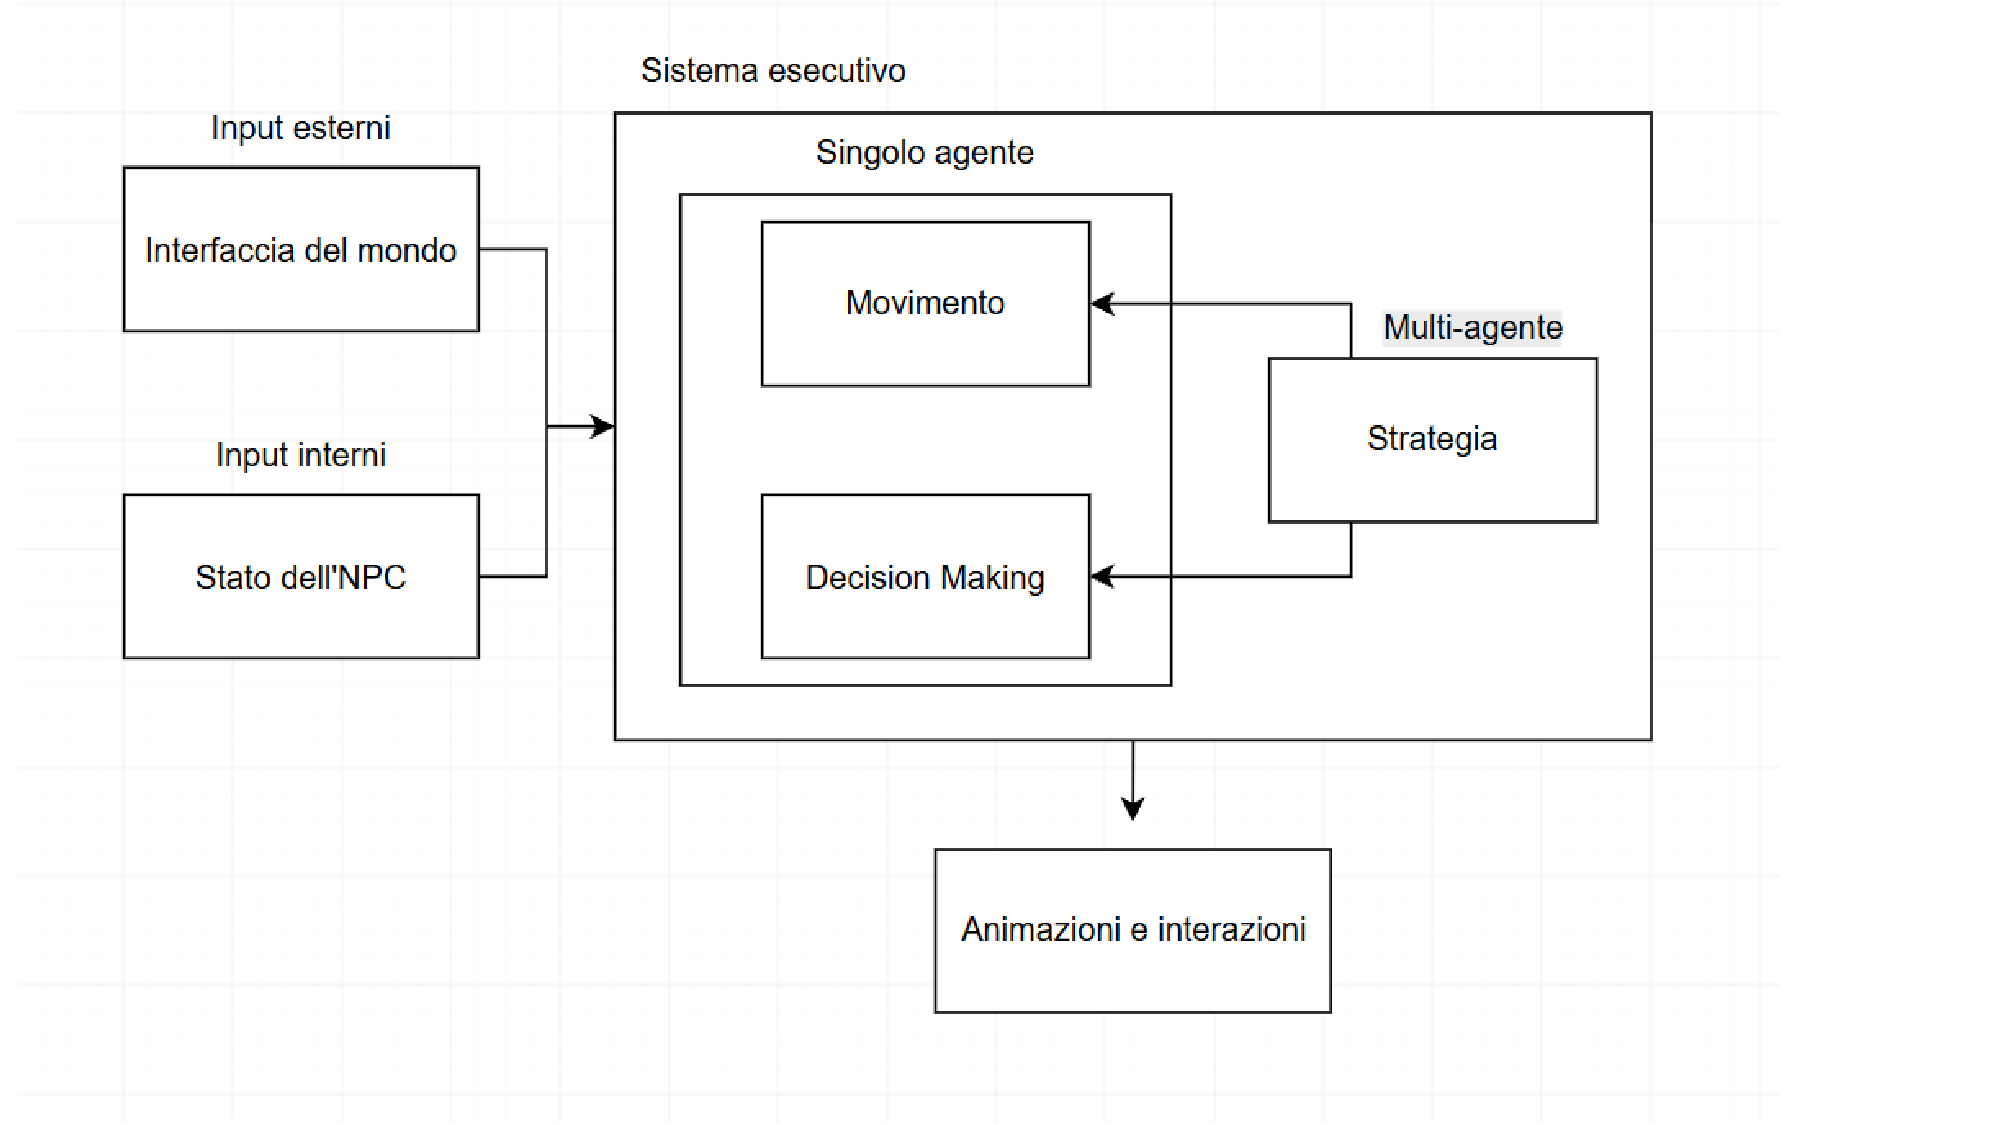
\includegraphics[width=1\textwidth]{figure/moduli_ia.pdf}
	\caption{Struttura a moduli dell'IA nei videogiochi. Figura adattata da \cite{millington2019artificial}.}
	\label{fig:moduli_ia}
\end{figure}

Il Movimento è definito come il modulo che calcola un certo tipo di percorso e coordina il movimento dell'NPC. Il Decision Making permette all'NPC di decidere quali azioni compiere tra quelle disponibili. La Strategia serve a coordinare i due moduli sopracitati per farli lavorare insieme ad altri agenti.
Non tutti i moduli sono necessari: \textit{Super Mario Galaxy}\cite{mariogalaxy} ha bisogno solo del modulo di movimento, dato che i nemici devono semplicemente inseguire il giocatore. Altri giochi d'azione più complicati come \textit{Dark Souls}\cite{darksouls} richiedono decisioni più complesse — attaccare, parare, muoversi o curarsi — ma non tengono conto delle azioni degli altri nemici, rendendo superflua la Strategia. Tutto ciò rientra nelle scelte di design: ogni videogioco vuole trasmettere emozioni diverse e offrire un diverso grado di sfida.
AmbraIA opera soprattutto sul campo del Decision Making, cercando di non coprire un genere preciso ma di creare un'IA che possa rendere gli NPC credibili in scene 3D differenti. Il Decision Making viene affrontato principalmente tramite due strutture: gli alberi decisionali e le macchine a stati finiti.

\subsection{Alberi decisionali}

Non entrando troppo nei particolari, gli alberi decisionali sono strutture dati che vengono percorse ogni volta che deve essere presa una decisione. Sono formati da un insieme di nodi e da archi, cioè collegamenti direzionati tra due nodi che rappresentano le decisioni. Gli alberi sono caratterizzati dall'assenza di cicli. Le decisioni finali sono rappresentate dai nodi foglia, cioè nodi senza archi uscenti.
Non appena c'è bisogno di prendere una decisione, l'albero viene percorso a partire dal suo nodo iniziale, detto radice. Viene percorso un arco piuttosto che un altro a seconda degli input che l'agente riceve, come la percezione del mondo esterno o il suo stato interno, ad esempio fame o stanchezza. Una volta arrivati al nodo foglia, la decisione è stata presa e si esegue l'azione designata, come mostrato in Figura \ref{fig:alberodecisionale}.

% TODO: \usepackage{graphicx} required
\begin{figure}[h]
	\centering
	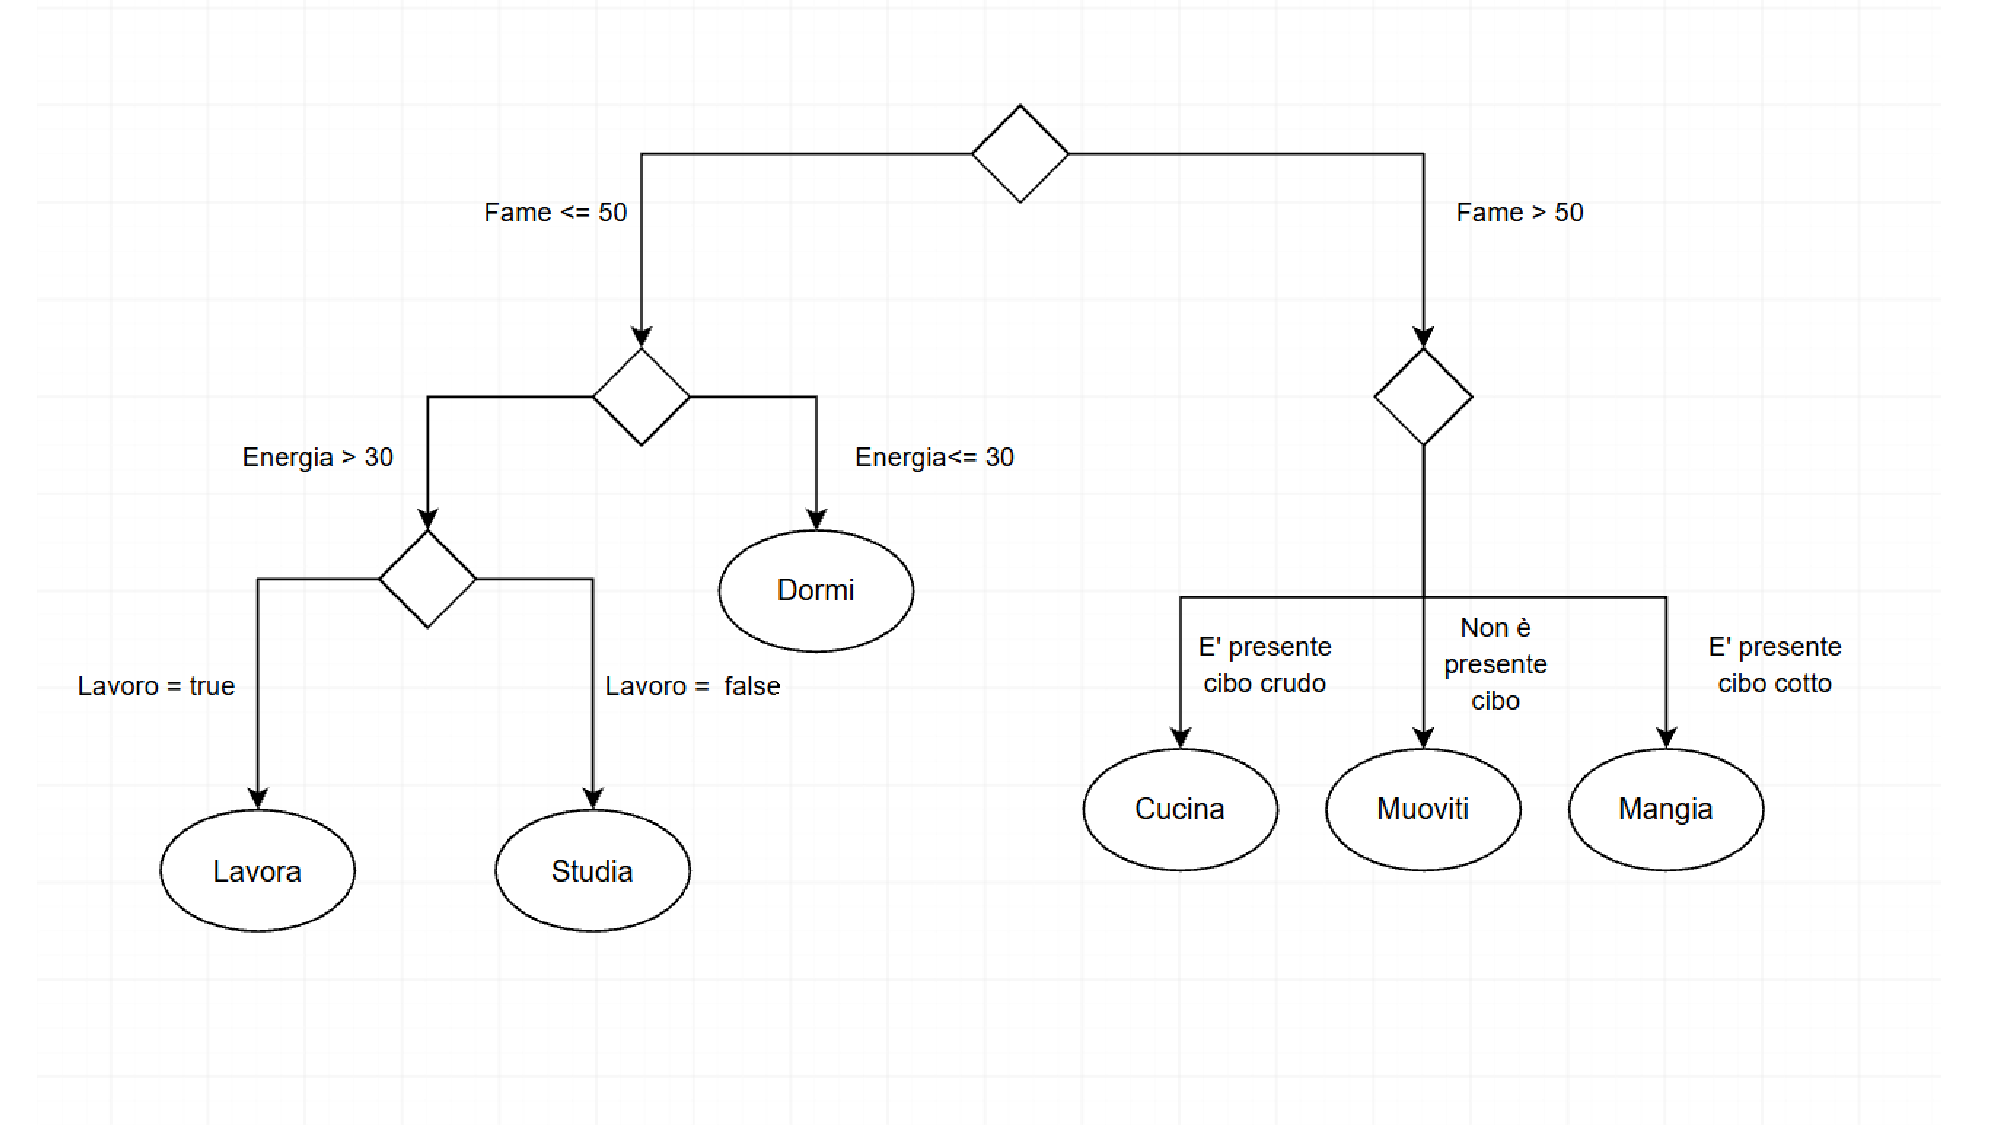
\includegraphics[width=1.1\textwidth]{figure/albero_decisionale}
	\caption{Esempio di albero decisionale per un NPC.}
	\label{fig:alberodecisionale}
\end{figure}

\subsection{Macchine a stati finiti}

Le macchine a stati finiti sono formalmente definite come una quintupla composta da:

\begin{itemize}
	\item Un insieme di stati $Q$
	\item Un alfabeto $\Sigma$
	\item Uno stato iniziale $q_0$
	\item Un insieme di stati finali $Q_f$
	\item Una funzione di transizione $\delta: Q \times \Sigma \rightarrow Q$
\end{itemize}

Nel contesto videoludico gli stati rappresentano una situazione in cui si trova l'NPC (in guardia, affamato, impaurito) che lo porta ad agire in un certo modo. Lo stato iniziale è la situazione di partenza dell'NPC. L'alfabeto rappresenta una serie di input. La funzione di transizione controlla se una condizione si verifica in un certo stato e, se ciò avviene, cambia lo stato dell'NPC. Gli stati finali rappresentano situazioni in cui l'NPC ha raggiunto un obiettivo o ha completato un comportamento. Le decisioni vengono quindi prese in base allo stato in cui si trova l'NPC in un determinato momento, come mostrato in Figura \ref{fig:fsm}.

\begin{figure}[h]
	\centering
	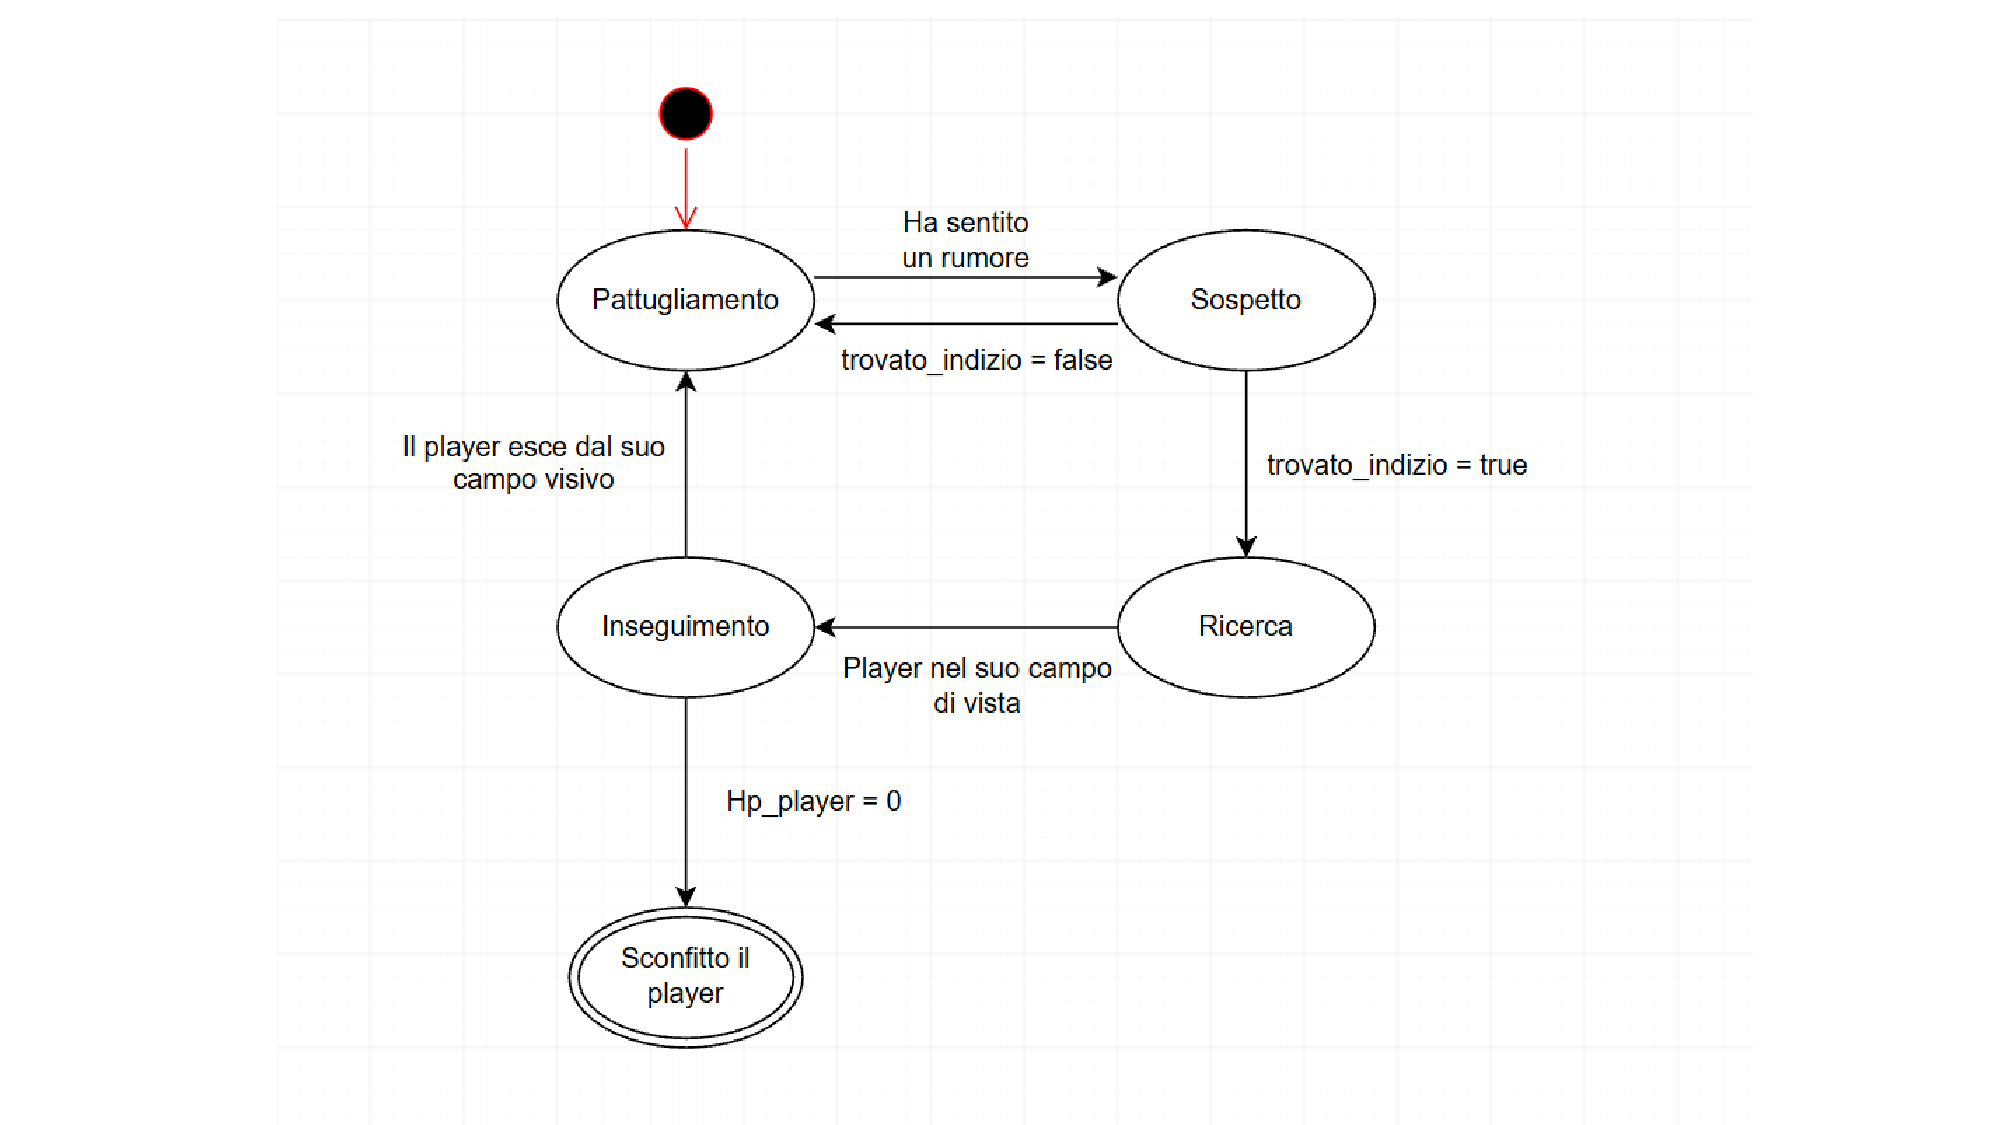
\includegraphics[width=0.91\textwidth]{figure/fsm.pdf}
	\caption{Esempio di macchina a stati finiti per un NPC.}
	\label{fig:fsm}
\end{figure}

\subsection{Limiti degli approcci tradizionali}

Questi approcci hanno molti vantaggi: sono strutturalmente semplici, possono essere trattati con valori primitivi e si possono combinare tra loro. Il limite più grande è la staticità di queste strutture: sono estremamente specifiche per il sistema in cui vengono implementate e non tengono conto delle azioni passate. Inoltre, ogni nuovo comportamento richiede la modifica manuale di stati, transizioni o rami dell'albero, rendendo difficile l'adattamento a contesti non previsti in fase di progettazione.

\section{Gli LLM nei videogiochi: opportunità e sfide}

L'intelligenza artificiale generativa e i Large Language Model rappresentano uno dei più grandi risultati dell'informatica moderna. Ormai gli LLM si sono introdotti nella maggior parte degli ambiti, lavorativi e non. Gli LLM sono modelli linguistici addestrati su enormi quantità di dati, che generano principalmente testo, ma si sta puntando sempre di più verso modelli General Purpose, in grado di generare anche immagini, audio, video e altro ancora.

\subsection{LLM come strumenti per lo sviluppo di videogiochi}

Anche nel mondo dei videogiochi gli LLM sono sbarcati, aiutando gli sviluppatori a creare strumenti che facilitano lo sviluppo. Un esempio è il progetto ``LLMR: Real-time Prompting of Interactive Worlds using Large Language Models'' di De La Torre et al. \cite{delatorre2024llmr}. LLMR è un framework per la creazione di asset e scene 3D che utilizza un modello linguistico per la generazione di questi asset. Nell'architettura descritta nel paper è importante l'approccio human in the loop: l'utente inizia una conversazione con il modello per fornire tutte le informazioni necessarie alla generazione degli asset. A questo punto l'LLM genera i file C\# che descrivono i vari elementi della scena. Una volta generati gli asset, l'utente può chiedere al modello modifiche automatiche oppure agire manualmente su di essi, prima di generare la scena completa.

\subsection{LLM per il controllo degli NPC}

Gli LLM inoltre assistono anche nella creazione di NPC. I comportamenti umani sono molto complessi, frutto di processi cognitivi articolati che comprendono l'analisi di ricordi ed esperienze passate, la percezione del mondo e lo stato fisiologico ed emotivo. I videogiochi che vogliono simulare i comportamenti umani, anche solo in parte, utilizzano per la maggior parte macchine a stati finiti enormi e molto specifiche per il gioco sviluppato; un esempio già citato è \textit{Tomodachi Life} \cite{tomodachilife}. Gli LLM possono essere utilizzati per semplificare queste architetture.

Nel paper scientifico ``LLM-Driven NPCs: Cross-Platform Dialogue System for Games and Social Platforms'' di Song \cite{song2025llmnpc} viene proposto un prototipo di NPC che dialoga tramite LLM con il giocatore sia in-game tramite Unity, sia fuori dal gioco su Discord. Parlare nel gioco aumenta un parametro che indica il gradimento dell'NPC, cioè il grado di familiarità tra il giocatore e l'NPC. Più il gradimento è alto, più l'NPC sarà confidente verso il giocatore. In questo caso l'LLM ha il solo compito di generare output testuali in base agli input testuali del giocatore.

I Large Language Model però sono stati usati anche per elaborare decisioni più complesse, come in ``Generative Agents: Interactive Simulacra of Human Behavior'' di Park et al. \cite{park2023generative}, in cui viene progettata e implementata un'architettura che simula una cittadina di persone, le quali interagiscono tra loro, hanno la loro routine e la loro personalità. L'architettura cerca di simulare alcuni processi cognitivi della mente umana, come il deposito di ricordi in un database, l'estrazione di ricordi in base alla loro importanza e recenza, o la riflessione periodica sulle proprie azioni. Questo è un esempio di IA di strategia e decision making, poiché gli abitanti della cittadina interagiscono tra loro e prendono decisioni in base al mondo circostante e allo stato dell'NPC.

\subsection{Sfide e limiti degli LLM}

Nonostante le opportunità offerte, gli LLM presentano anche diverse criticità. Possono essere soggetti ad allucinazioni, generando informazioni non veritiere o incoerenti con il contesto; i tempi di esecuzione possono essere elevati, soprattutto quando il modello viene eseguito localmente; inoltre, in assenza di un'architettura adeguata, tendono a ripetere le stesse risposte o gli stessi comportamenti. Queste sfide rendono necessario progettare sistemi che affianchino all'LLM componenti deterministiche in grado di gestire memoria, coerenza e affidabilità.

AmbraIA prende ispirazione dalle architetture sopraccitate e cerca di creare un NPC che possa interagire in un ambiente 3D di Unity, prendendo decisioni coerenti con il suo stato fisiologico e la sua percezione dell'ambiente. AmbraIA non è una struttura pensata per un videogioco o un ambiente specifico, grazie a un sistema semi-automatico di matching tra GameObject e interazioni/animazioni definite dallo sviluppatore. L'LLM viene utilizzato da AmbraIA per pianificare le azioni, mappare le azioni in C\# e generare riflessioni periodiche. Tutti questi aspetti vengono approfonditi nel Capitolo 3.

\chapter{L'architettura di AmbraIA}

AmbraIA è un'architettura cognitiva per agenti autonomi in ambienti 3D, supportata da modelli linguistici generativi. Questa architettura è divisa in vari moduli, ognuno con il compito di preparare i dati per il modulo successivo; il risultato finale viene inviato a Unity, dove prende la forma di uno script C\# che permette all'agente di muoversi e interagire con la scena. Prima di descrivere in dettaglio ogni modulo, partiamo dalla definizione del problema dell'NPC che interagisce con l'ambiente e dalla descrizione dell'ambiente stesso.

\section{Specifica PEAS}

Per descrivere formalmente l'agente e il suo ambiente, si utilizza il modello PEAS (Performance, Environment, Actuators, Sensors), uno standard nella progettazione di agenti intelligenti.

\begin{description}
	\item[Performance] Le misure di prestazione adottate per valutare l'operato dell'agente sono:
	\begin{itemize}
		\item Coerenza delle azioni con lo stato fisiologico
		\item Varietà dei comportamenti nel tempo
		\item Tasso di successo della compilazione del codice C\# generato
		\item Tempo di risposta del server, cioè la latenza tra richiesta e piano generato
		\item Adattabilità a scene nuove, cioè il sistema configura scene non preconfigurate
	\end{itemize}
	
	\item[Environment] Gli elementi che formano l'ambiente sono:
	\begin{itemize}
		\item Una scena 3D Unity con oggetti interagibili (cibo, mobili, oggetti decorativi)
		\item Proprietà specifiche per ogni oggetto (nome, tag, azione disponibile, effetti fisiologici)
		\item Lo stato fisiologico dell'NPC (fame e stanchezza), che evolve dinamicamente nel tempo
	\end{itemize}
	
	\item[Actuators] Gli attuatori disponibili dall'agente sono:
	\begin{itemize}
		\item Movimento verso un oggetto (\texttt{MoveToTargetAndWait})
		\item Interazione con un oggetto (\texttt{InteractWithAndWait})
		\item Modifica dello stato fisiologico come conseguenza delle interazioni
	\end{itemize}
	
	\item[Sensors] I sensori attraverso i quali l'agente riceve input percettivi sono:
	\begin{itemize}
		\item Lista degli oggetti nel raggio di percezione (nome, distanza, azione, effetto)
		\item Stato fisiologico corrente (fame, stanchezza)
		\item Cronologia delle azioni più importanti e recenti
		\item Memoria a lungo termine
	\end{itemize}
\end{description}

\section{Caratteristiche dell'ambiente}

L'ambiente in cui opera AmbraIA presenta le seguenti caratteristiche:

\begin{description}
	\item[Singolo agente] Il problema è modellato come un problema a singolo agente. Non sono presenti altri NPC o agenti concorrenti durante l'esecuzione, sebbene l'architettura sia predisposta per future estensioni multi-agente.
	
	\item[Parzialmente osservabile] L'agente percepisce solo gli oggetti entro un raggio di percezione configurabile, non l'intera scena. Inoltre non ha accesso diretto allo stato interno degli oggetti (ad esempio, non sa se un cibo è già stato consumato).
	
	\item[Semi-deterministico] Le interazioni con gli oggetti hanno effetti deterministici: mangiare una mela riduce sempre la fame di un valore fisso. Tuttavia, il processo decisionale basato su LLM introduce non-determinismo nella scelta delle azioni.
	
	\item[Sequenziale] Il processo decisionale non è suddiviso in episodi indipendenti, ma consiste in una sequenza continua di pianificazione, esecuzione e aggiornamento della memoria. Le decisioni hanno conseguenze a lungo termine perché influenzano i ricordi che guideranno le scelte future.
	
	\item[Statico] L'ambiente è statico durante l'esecuzione di un piano: gli oggetti non cambiano posizione o proprietà mentre l'NPC esegue le azioni. Lo stato fisiologico dell'NPC, invece, si modifica continuamente nel tempo.
	
	\item[Discreto] Lo spazio degli stati è discreto. Le azioni disponibili sono in numero finito e lo stato fisiologico è rappresentato da valori normalizzati tra 0 e 1.
\end{description}

\section{Analisi del problema}

Il problema può essere formalizzato come un problema di pianificazione continua in un ambiente parzialmente osservabile, dove ogni stato è definito dalla combinazione di posizione dell'NPC, stato fisiologico, oggetti percepiti e contenuto del Memory Stream, cioè della memoria persistente.

\begin{description}
	\item[Stati] Configurazione corrente dell'NPC: posizione, fame, stanchezza e ricordi accumulati.
	\item[Stato iniziale] NPC posizionato nella scena con fame e stanchezza iniziali e Memory Stream vuoto.
	\item[Azioni] Movimento verso un oggetto oppure interazione con un oggetto.
	\item[Spazio degli stati] Tutte le possibili combinazioni di posizioni, livelli fisiologici, oggetti percepiti e ricordi accumulati.
	\item[Test obiettivo] Non esiste uno stato obiettivo finale. L'NPC deve mantenere un comportamento coerente e adattivo indefinitamente.
\end{description}

Il problema presenta le seguenti caratteristiche:

\begin{itemize}
	\item Spazio degli stati potenzialmente illimitato, a causa della crescita continua del Memory Stream.
	\item Assenza di una soluzione ottima calcolabile: non esiste un comportamento ``perfetto''.
	\item Necessità di bilanciare bisogni multipli simultaneamente (fame e stanchezza).
	\item Necessità di mantenere coerenza temporale, senza contraddire i ricordi e le riflessioni.
\end{itemize}

Per questi motivi, il problema non può essere risolto tramite alberi decisionali predefiniti o macchine a stati finite tradizionali, ma risulta adatto all'uso di LLM combinati con un'architettura di memoria, retrieval e riflessione.

\section{Il lato Unity di AmbraIA}

AmbraIA è suddivisa principalmente in due macro moduli: il lato Unity e il lato server. Il lato Unity ha il compito di raccogliere i dati di input dall'ambiente e di gestire i dati di output, cioè le azioni che l'NPC deve eseguire. È composto da quattro sotto-moduli principali, implementati come script C\#:

\begin{itemize}
	\item \texttt{NPCController}: permette all'NPC di muoversi e interagire con gli oggetti della scena.
	\item \texttt{SceneAnalyzer}: analizza la scena e invia i dati al server.
	\item \texttt{InteractableObject}: permette ai GameObject di diventare interagibili.
	\item \texttt{RuntimeCompiler}: compila a runtime il codice C\# generato dal server e lo attacca all'NPC.
\end{itemize}

La Figura \ref{fig:lato_unity} mostra una panoramica del lato Unity.

\begin{figure}[h]
	\centering
	\hspace*{-5cm}
	
\includegraphics[width=1.5\textwidth]{lato_unity.pdf}
	\caption{Panoramica del lato Unity di AmbraIA.}
	\label{fig:lato_unity}
\end{figure}

\subsection{NPCController}

Questo componente permette di eseguire il piano di azioni compilato dal \texttt{Runtime\-Compiler}. Fornisce i metodi per far muovere l'NPC e per interagire con gli oggetti interagibili, attivando animazioni ed effetti. Il movimento viene gestito tramite il NavMesh, una rappresentazione semplificata della geometria della scena che indica le aree calpestabili e gli ostacoli. In questo modo l'agente può calcolare percorsi validi evitando muri e oggetti non attraversabili. Una volta arrivato nei pressi dell'oggetto con cui interagire, l'NPC attiva l'animazione e l'effetto specifico dell'interazione, descritti dall'\texttt{InteractableObject}.

L'\texttt{NPCController} contiene inoltre i dati dello stato interno dell'NPC, che in questo caso sono fame e stanchezza: questi rappresentano i bisogni prioritari che l'NPC deve soddisfare. Entrambi sono rappresentati da valori decimali compresi tra 0 e 1, dove 0 indica uno stato ottimale e 1 un bisogno critico. Fame e stanchezza aumentano gradualmente nel tempo: la fame cresce costantemente, mentre la stanchezza aumenta più rapidamente quando l'NPC si muove e più lentamente quando è fermo. Le interazioni con gli oggetti possono ridurre o aumentare questi valori.


\subsection{InteractableObject}

\texttt{InteractableObject} è il modulo che rappresenta l'interazione e viene associato ai GameObject che possono essere interagiti. Contiene quattro informazioni principali:

\begin{itemize}
	\item il nome dell'interazione (ad esempio ``Usa'' o ``Mangia'');
	\item l'animazione da attivare;
	\item la coordinata spaziale in cui l'NPC deve trovarsi per interagire con quell'oggetto;
	\item l'effetto, cioè il valore di modifica di fame e stanchezza dopo l'interazione.
\end{itemize}

Se a un GameObject non è associato un \texttt{InteractableObject}, questo non verrà considerato come oggetto interagibile. Il componente include inoltre un campo opzionale, \texttt{oggettoDaAttivare}, che permette di attivare un secondo GameObject al termine dell'interazione: questo consente di realizzare interazioni a più step, come nel caso del fornello che, una volta usato, fa apparire un piatto cotto.


\subsection{SceneAnalyzer}

\texttt{SceneAnalyzer} è il modulo che ha il compito di inviare i dati della scena al server tramite richiesta HTTP con endpoint \texttt{/npc/decide}. Il componente definisce il raggio di percezione dell'NPC: tutti gli oggetti interagibili che ricadono entro questo raggio vengono inseriti in una lista, dove ognuno è descritto da nome, tag, azione disponibile, effetto fisiologico e distanza dall'NPC. Nel calcolo dell'effetto, \texttt{SceneAnalyzer} legge direttamente i valori di \texttt{fameEffect} ed \texttt{energyEffect} dall'\texttt{InteractableObject} e li classifica come \textit{hunger}, \textit{energy}, \textit{both} o \textit{none}.

Oltre agli oggetti vicini, l'analyzer invia al server anche lo stato fisiologico corrente dell'NPC, le ultime azioni eseguite e le riflessioni accumulate. Se l'NPC ha una fame o una stanchezza maggiore o uguale a 0.7, l'Analyzer notificherà la criticità. In questo modo il server ha tutte le informazioni necessarie per pianificare le azioni successive. Se il file C\# generato dal server contiene un errore di compilazione, lo \texttt{SceneAnalyzer} notifica l'errore al server e richiede un nuovo tentativo: questo meccanismo di retry può avvenire fino a un massimo di tre volte, sia per errori di compilazione sia per errori HTTP.

Quando un'azione viene completata, lo \texttt{SceneAnalyzer} invia una notifica al server tramite l'endpoint \texttt{/npc/action-done}, in modo che l'azione venga registrata nella memoria a lungo termine. Questa comunicazione avviene separatamente dalla richiesta di pianificazione, così il Memory Stream rimane sempre aggiornato.

\subsection{RuntimeCompiler}

\texttt{RuntimeCompiler} ha il compito di compilare il piano d'azione, scritto in codice sorgente C\# e generato dal server, per poi attaccarlo all'NPC. Unity normalmente compila tutto il codice a tempo di build, ma in questo caso il codice non esiste finché il server non lo genera, quindi è necessario compilarlo durante l'esecuzione del gioco. Per farlo, il componente utilizza Roslyn, il compilatore C\# ufficiale di Microsoft.

Il processo avviene interamente in memoria: se la compilazione ha successo, la classe generata viene attaccata al GameObject dell'NPC, sostituendo quella del piano precedente. Se invece la compilazione fallisce, \texttt{RuntimeCompiler} restituisce una stringa con gli errori riscontrati, che \texttt{SceneAnalyzer} invierà al server per richiedere una correzione.

\section{Il lato server di AmbraIA}

Il lato server ha il compito di elaborare i dati ricevuti da Unity e di generare un piano d'azione sotto forma di file C\#, che viene poi rimandato indietro. È stato implementato interamente in Python. Per orchestrare i diversi sotto-moduli del server ho scelto di utilizzare LangGraph, un framework open source sviluppato da LangChain. LangGraph permette di costruire workflow complessi con agenti di AI generativa, gestendo in modo chiaro il flusso di dati tra un modulo e l'altro. Il server è composto da sei moduli principali:

\begin{itemize}
	\item \texttt{Memory Stream}: memoria persistente che registra tutte le esperienze dell'NPC.
	\item \texttt{Retrieval}: recupera dal Memory Stream i ricordi più rilevanti per la situazione attuale.
	\item \texttt{Planner}: genera un piano d'azione gerarchico basato sulla scena, sui ricordi e sulle riflessioni, tramite una chiamata a un LLM.
	\item \texttt{Builder}: traduce il piano in codice C\# eseguibile da Unity, sempre tramite LLM.
	\item \texttt{Inspector}: valida il codice generato, verificando che non contenga errori o placeholder.
	\item \texttt{Reflector}: analizza periodicamente le esperienze recenti e produce riflessioni di alto livello, tramite una chiamata all'LLM.
\end{itemize}
La Figura \ref{fig:lato_server} mostra una panoramica del lato server.

\begin{figure}[H]
	\centering
	
\includegraphics[width=1.1\textwidth]{lato_server.pdf}
	\caption{Panoramica del lato server di AmbraIA.}
	\label{fig:lato_server}
\end{figure}

\subsection{Memory Stream}

Il Memory Stream rappresenta la memoria permanente dell'architettura. Consiste in un file JSON in cui sono raccolti tutti i ``ricordi'' dell'NPC, cioè le sue azioni passate. Questo serve a simulare i ricordi umani e aiuta a evitare comportamenti ripetitivi, incoerenti, o che in passato hanno portato a effetti negativi. Ogni ricordo è composto da:

\begin{itemize}
	\item \texttt{id}: identificativo alfanumerico del ricordo;
	\item \texttt{content}: descrizione testuale del ricordo;
	\item \texttt{timestamp}: momento in cui è avvenuto il ricordo;
	\item \texttt{importance}: numero intero da 1 a 10 che indica l'importanza del ricordo. Non tutte le esperienze hanno lo stesso valore: mangiare una mela quando si ha fame è più significativo che mangiarla quando si è già sazi. Per questo il punteggio viene assegnato dall'LLM al momento della creazione del ricordo, valutando l'impatto sullo stato fisico, la novità dell'evento e l'utilità per le decisioni future. Questo valore influenza il Retrieval, dando più peso ai ricordi ritenuti più importanti;
	\item \texttt{type}: tipo del ricordo, che può essere \texttt{action} o \texttt{reflection};
	\item \texttt{embedding}: vettore di 768 numeri che rappresenta il significato del testo. Viene generato tramite \texttt{nomic-embed-text}, un modello eseguito localmente che trasforma una frase in una rappresentazione numerica. Due frasi con significato simile avranno vettori vicini nello spazio, anche se non condividono le stesse parole: ad esempio ``Ho mangiato una mela'' e ``Ho consumato del cibo'' producono embedding molto simili. Questo permette al Retrieval di confrontare i ricordi con la situazione attuale in modo semantico, senza dover cercare parole chiave.
\end{itemize}

La Lista \ref{lst:ricordo} mostra un esempio di ricordo salvato nel Memory Stream.

\begin{lstlisting}[style=jsonstyle, caption={Esempio di ricordo nel Memory Stream.}, label={lst:ricordo}]
	{
		"id": "mem_a3f2c1d4",
		"content": "Mangia su Mela",
		"timestamp": 1726000000.0,
		"importance": 6,
		"type": "action",
		"embedding": [0.12, -0.34, 0.78, "...altri 765 valori..."]
	}
\end{lstlisting}

Retriaval
\subsection{Retrieval}

Il Retrieval è il modulo che si occupa di recuperare dal Memory Stream i ricordi più utili per la situazione attuale. L'LLM, da solo, non può ricevere l'intera memoria dell'NPC: dopo diverse ore di gioco il numero di ricordi accumulati diventa troppo elevato per essere inserito in un singolo prompt. È quindi necessario un meccanismo di selezione che scelga solo i ricordi più rilevanti; d'altronde anche la mente umana estrae specifici ricordi in specifiche situazioni.

Il Retrieval estrae i primi dieci ricordi in base a un punteggio calcolato combinando tre fattori:

\begin{itemize}
	\item \textbf{Recency}: quanto è recente il ricordo. Un'esperienza appena vissuta è spesso più utile e adatta al contesto attuale di una di diverse ore fa. Il decadimento è esponenziale, così i ricordi invecchiano rapidamente all'inizio e più lentamente col passare del tempo;
	\item \textbf{Importance}: quanto è importante il ricordo, secondo il punteggio da 1 a 10 assegnato dall'LLM al momento della creazione del ricordo;
 	\item \textbf{Relevance}: quanto il ricordo è semanticamente simile alla situazione attuale. Per calcolarla, ogni ricordo e la situazione corrente vengono trasformati in embedding, cioè vettori di 768 numeri che ne rappresentano il significato. Due testi con significato simile producono vettori vicini nello spazio, anche se non condividono le stesse parole. La similarità tra i due vettori si misura tramite la similarità del coseno, che restituisce un valore tra 0 e 1: valori vicini a 1 indicano che il ricordo è semanticamente pertinente alla situazione attuale, valori vicini a 0 indicano che è poco rilevante.
\end{itemize}

Il punteggio finale è una combinazione pesata dei tre fattori, secondo la formula:

\begin{equation}
	\text{score} = \alpha_{\text{recency}} \cdot \text{recency} + \alpha_{\text{importance}} \cdot \text{importance} + \alpha_{\text{relevance}} \cdot \text{relevance}
\end{equation}

dove i pesi sono $\alpha_{\text{recency}} = 0.3$, $\alpha_{\text{importance}} = 0.3$ e $\alpha_{\text{relevance}} = 0.4$. Il peso maggiore dato alla relevance riflette l'importanza della pertinenza contestuale: se l'NPC ha fame, un ricordo legato al cibo è più utile di un ricordo recente ma su un argomento diverso.

La formula completa per il calcolo del punteggio, tenendo conto di tutti e tre i fattori, è la seguente:

\begin{equation}
	\text{score}(m) = \alpha_r \cdot \frac{1}{1 + \lambda \cdot \Delta t_m} + \alpha_i \cdot \frac{i_m}{10} + \alpha_v \cdot \cos(\vec{e}_m, \vec{e}_q)
\end{equation}

dove:
\begin{itemize}
	\item $\Delta t_m$ è il tempo trascorso (in ore) dal momento in cui il ricordo $m$ è stato creato;
	\item $\lambda = 0.99$ è il fattore di decadimento;
	\item $i_m$ è l'importance del ricordo $m$;
	\item $\vec{e}_m$ è l'embedding del ricordo $m$;
	\item $\vec{e}_q$ è l'embedding della query, cioè la descrizione della situazione attuale.
\end{itemize}

I dieci ricordi con il punteggio più alto vengono passati al Planner come contesto storico, così che il piano generato tenga conto delle esperienze passate dell'NPC.

\subsection{Planner}

Il Planner è il primo nodo del grafo a chiamare l'LLM. Il suo compito è generare un piano d'azione in linguaggio naturale, che verrà poi utilizzato come input dal nodo successivo, il Builder. Riceve come input i ricordi estratti dal Retrieval, tutti gli oggetti interagibili presenti nella scena, lo stato fisiologico corrente dell'NPC, le azioni recenti e le riflessioni accumulate.

Il formato della risposta è un piano d'azione composto da un obiettivo principale e da un massimo di tre sotto-obiettivi, ciascuno con una priorità (alta, media o bassa). Ogni sotto-obiettivo descrive l'azione da compiere e l'oggetto su cui agire, in modo che il Builder comprenda in che ordine devono essere eseguite le azioni.

La Lista \ref{lst:piano} mostra un esempio di piano generato dal Planner.

\begin{lstlisting}[style=jsonstyle, caption={Esempio di piano generato dal Planner.}, label={lst:piano}]
	GOAL: Mantenermi in salute
	
	SOTTO-OBIETTIVO 1 [PRIORITA: ALTA]: Soddisfare la fame
	- Azione: Vai a Mela
	- Azione: Mangia su Mela
	
	SOTTO-OBIETTIVO 2 [PRIORITA: MEDIA]: Riposarmi
	- Azione: Vai a Sedia
	- Azione: Siediti su Sedia
\end{lstlisting}

Il Planner tiene conto di alcune regole fondamentali: se la fame o la stanchezza superano la soglia critica di 0.7, il bisogno corrispondente diventa la priorità assoluta; le azioni già eseguite di recente non tendono ad essere ripetute; se le riflessioni suggeriscono di variare il comportamento, il piano deve riflettere questo cambiamento; se non ci sono bisogni urgenti, l'NPC deve esplorare nuovi oggetti o attività.

\subsection{Builder}

Il Builder converte il piano d'azione in linguaggio naturale, generato dal Planner, in codice C\# eseguibile su Unity. Come il Planner, riceve in input la lista degli oggetti interagibili con le rispettive azioni valide e le distanze dall'NPC. In base alle azioni decise dal Planner, il Builder mappa ogni interazione con un massimo di due istruzioni:

\begin{itemize}
	\item \texttt{MoveToTargetAndWait}: muove l'NPC verso l'oggetto target, se questo si trova a una distanza superiore a un'unità;
	\item \texttt{InteractWithAndWait}: obbligatoria per far avvenire l'interazione, avvia l'animazione e applica l'effetto fisiologico corrispondente.
\end{itemize}

La Lista \ref{lst:codice_generato} mostra un esempio di codice C\# generato dal Builder.

\begin{lstlisting}[style=jsonstyle, caption={Esempio di codice C\# generato dal Builder.}, label={lst:codice_generato}]
	using UnityEngine;
	using System.Collections;
	
	public class AiAction : MonoBehaviour
	{
		void Start()
		{
			StartCoroutine(ExecutePlan());
		}
		
		IEnumerator ExecutePlan()
		{
			NPCController controller = GetComponent<NPCController>();
			if (controller == null) yield break;
			
			// SOTTO-OBIETTIVO 1: Soddisfare la fame [PRIORITA: ALTA]
			yield return StartCoroutine(controller.MoveToTargetAndWait("Mela"));
			yield return StartCoroutine(controller.InteractWithAndWait("Mela", "Mangia"));
			
			// SOTTO-OBIETTIVO 2: Riposarmi [PRIORITA: MEDIA]
			yield return StartCoroutine(controller.MoveToTargetAndWait("Sedia"));
			yield return StartCoroutine(controller.InteractWithAndWait("Sedia", "Siediti"));
			
			Destroy(this);
			yield break;
		}
	}
\end{lstlisting}

Il Builder opera in modalità deterministica, con temperatura impostata a zero, per ridurre al minimo la variabilità dell'output. Il codice generato è vincolato a una struttura fissa: la classe deve chiamarsi \texttt{AiAction}, deve ereditare da \texttt{MonoBehaviour} e deve usare esclusivamente i due metodi esposti dall'\texttt{NPCController}. Al termine dell'esecuzione, la classe si autodistrugge tramite \texttt{Destroy(this)}, così che il componente non si accumuli sull'NPC tra un piano e il successivo.

\subsection{Inspector}

L'Inspector è l'ultimo nodo del grafo e ha il compito di controllare che il codice generato dal Builder non contenga errori gravi. Se il controllo fallisce, il codice viene rimandato al Builder per un ulteriore tentativo, fino a un massimo di tre.

L'Inspector verifica tre categorie di problemi:

\begin{itemize}
	\item \textbf{Placeholder}: controlla che il codice non contenga pseudo-codice, commenti al posto di istruzioni reali (es. \texttt{if (/* condizione */)}), oppure testi come ``TODO'' o ``da implementare'';
	\item \textbf{Nomi degli oggetti}: estrae i nomi degli oggetti usati nelle chiamate a \texttt{MoveToTargetAndWait} e \texttt{InteractWithAndWait} e verifica che corrispondano a oggetti realmente presenti nella scena;
	\item \textbf{Nomi dei componenti}: controlla che il nome del controller utilizzato nel codice sia corretto (ad esempio, che sia \texttt{NPCController} e non una variante inventata dall'LLM).
\end{itemize}

Può capitare che il codice contenga altri tipi di errore che l'Inspector non è in grado di rilevare, come errori di sintassi o di tipo. In questo caso, quando Unity tenta di compilare il codice, genera un errore e lo rispedisce al server. Il grafo riparte direttamente dal Builder, saltando Retrieval e Planner, e il Builder riceve l'errore nel prompt per correggere il codice. In questo modo, l'Inspector ha il compito principale di individuare gli errori immediati e di velocizzare il flusso di lavoro, evitando di far arrivare a Unity codice che sarebbe sicuramente scartato.

\subsection{Reflector}

Il Reflector non è un nodo del grafo, ma un modulo indipendente che viene eseguito ogni cinque azioni completate. Come input riceve i ricordi più recenti del Memory Stream, in particolare le ultime venti azioni e osservazioni. Il Reflector chiede all'LLM di generare una o più riflessioni di alto livello sui comportamenti recenti dell'NPC, identificando pattern, abitudini ricorrenti o comportamenti poco coerenti.

Le riflessioni generate vengono salvate nel Memory Stream come ricordi di tipo \texttt{reflection}, con un punteggio di importanza fissato a 9. In questo modo, grazie alla formula del Retrieval, tenderanno a essere recuperate spesso e a influenzare le pianificazioni successive; di conseguenza il Planner terrà conto di queste osservazioni.

La Lista \ref{lst:riflessione} mostra un esempio di riflessione generata dal Reflector.

\begin{lstlisting}[style=jsonstyle, caption={Esempio di riflessione generata dal Reflector.}, label={lst:riflessione}]
	L'NPC tende a mangiare sempre la stessa mela.
	Dovrebbe esplorare altre fonti di cibo disponibili nella scena.
\end{lstlisting}

\section{Configurazione scena}

AmbraIA prevede una configurazione della scena semi-automatica. L'utente deve inserire la proprietà \textit{static} sul pavimento e su tutti i GameObject che sono considerati ostacoli per il movimento. Deve poi creare dei Template per gli oggetti interagibili, creabili dal menù a tendina degli asset, in cui specifica nome, animazione ed effetto, più due campi opzionali dove può aggiungere delle parole chiave per il nome o per il tag degli oggetti. Ad esempio, se l'azione è ``siediti'' può inserire parole chiave come ``sedia, divano, letto, poltrona''.

A questo punto, dalla barra in alto, sotto la voce ``NPC'' può avviare l'analisi che mappa tutti gli oggetti con un tag come interagibili e associa a ciascuno un \texttt{InteractableObject} in base al template. L'associazione può avvenire in due modi: per corrispondenza di parole chiave, oppure, in mancanza di corrispondenza, tramite una chiamata all'LLM che, ricevendo la lista di oggetti e i template disponibili, deciderà a quale template associare ogni oggetto.

Perché l'NPC venga riconosciuto dal sistema, il suo GameObject deve avere un componente \texttt{NPCController} attaccato, oltre a \texttt{SceneAnalyzer}, \texttt{RuntimeCompiler}, \texttt{NavMeshAgent} e \texttt{Animator}. Il tool cerca un \texttt{NPCController} nella scena per verificare se l'NPC è già presente e, se non lo trova, lo istanzia automaticamente dalla posizione $(0,0,0)$.

A questo punto la scena è pronta, ma nulla vieta all'utente di apportare ulteriori modifiche alle interazioni o alle associazioni qualora non fosse soddisfatto del risultato.

\chapter{Sperimentazione e Risultati}

\section{Setup sperimentale}

L'architettura è stata testata principalmente su una singola scena che funge da soggiorno, contenente sei oggetti interagibili: un PC, una sedia, un divano, una console, un bicchiere di vino e una ciotola di cibo. La Tabella \ref{tab:setup} riassume i dettagli della configurazione utilizzata durante i test.

\begin{table}[H]
	\centering
	\caption{Configurazione del setup sperimentale.}
	\label{tab:setup}
	\begin{tabularx}{\textwidth}{|l|X|l|}
		\hline
		\textbf{Parametro} & \textbf{Valore} \\
		\hline
		\multicolumn{2}{|c|}{\textbf{Ambiente}} \\
		\hline
		Tipo di scena & Soggiorno/camera da letto \\
		Oggetti interagibili & 6 (PC, sedia, divano, console, bicchiere di vino, ciotola di cibo) \\
		\hline
		\multicolumn{2}{|c|}{\textbf{Template}} \\
		\hline
		Template creati & PC, Cibo, Videogioco, Bevande, Letto, Sedia, Libro \\
		\hline
		\multicolumn{2}{|c|}{\textbf{Modelli}} \\
		\hline
		Modello LLM & llama3.1 \\
		Modello di embedding & nomic-embed-text \\
		Dimensione embedding & 768 \\
		\hline
		\multicolumn{2}{|c|}{\textbf{Parametri fisiologici}} \\
		\hline
		Consumo fame passivo & 0.0007/s \\
		Consumo energia movimento & 0.007/s \\
		Consumo energia da fermo & 0.0004/s \\
		Soglia critica & 0.7 \\
		Cooldown pianificazione & 3.0s \\
		Ricordi recuperati (top-N) & 10 \\
		Pesi Retrieval & 0.3 recency, 0.3 importance, 0.4 relevance \\
		\hline
		\multicolumn{2}{|c|}{\textbf{Configurazione server}} \\
		\hline
		Intervallo Reflector & ogni 5 azioni \\
		Max tentativi Builder & 3 \\
		\hline
	\end{tabularx}
\end{table}

\newpage
La Figura \ref{fig:scena_test} mostra la scena utilizzata durante i test, con l'NPC al centro della scena.

\begin{figure}[H]
	\centering
	
\includegraphics[width=0.8\textwidth]{scena.pdf}
	\caption{La scena di test con l'NPC e gli oggetti interagibili.}
	\label{fig:scena_test}
\end{figure}

\section{Criteri di valutazione}

Per valutare i risultati dell'architettura bisogna considerare principalmente metriche qualitative rispetto a quantitative, poiché il comportamento di un NPC non è misurabile con metriche tradizionali come accuracy o precision. La credibilità e la coerenza di un agente emergono dall'osservazione del comportamento nel tempo, non dal calcolo di un singolo valore numerico. Fanno eccezione i tempi di risposta e il tasso di successo della compilazione, che sono intrinsecamente quantitativi. Le metriche utilizzate per valutare il sistema sono riassunte nella Tabella \ref{tab:criteri}.

\begin{table}[h]
	\centering
	\caption{Criteri di valutazione adottati.}
	\begin{tabularx}{\textwidth}{|l|X|l|}
		\hline
		\label{tab:criteri}
		\textbf{Criterio} & \textbf{Descrizione} & \textbf{Tipo} \\
		\hline
		Coerenza delle azioni & L'NPC si definisce coerente se compie azioni che riflettono il suo stato fisiologico, ad esempio mangia se ha fame, oppure si intrattiene o studia se non ha bisogno di mangiare o riposare. & Qualitativa \\
		\hline
		Varietà comportamentale & L'NPC ha una buona varietà comportamentale se non tende a ripetere le stesse azioni in presenza di oggetti diversi ma con effetto simile. & Qualitativa \\
		\hline
		Tasso di successo compilazione & Numero di compilazioni riuscite diviso il numero di compilazioni totali. & Quantitativa \\
		\hline
		Latenza & Differenza di tempo tra la richiesta e la risposta. & Quantitativa \\
		\hline
		Adattabilità & Il sistema si adatta a nuove scene. & Qualitativa \\
		\hline
	\end{tabularx}
\end{table}